% Poster capricorne asiatique (M1, 2023), refait en 2026. Format A0.
% Compiler dans outils/rapports/capricorne : Rscript figures.R && ../compiler.sh capricorne
\documentclass{article}
\usepackage[paperwidth=841mm,paperheight=1189mm,margin=0mm]{geometry}
\usepackage{fontspec}
\setmainfont{Source Sans 3}[BoldFont={Source Sans 3 SemiBold}]
\newfontfamily\titre{Lora}[BoldFont={Lora SemiBold},ItalicFont={Lora},ItalicFeatures={FakeSlant=0.18}]
\usepackage[french]{babel}
\usepackage{xcolor,graphicx,tikz,enumitem,csquotes}
\usepackage[hidelinks]{hyperref}
\usepackage[style=authoryear,maxcitenames=2,backend=bibtex,giveninits=true,dashed=false]{biblatex}
\DefineBibliographyExtras{french}{\renewcommand*{\mkbibnamefamily}[1]{#1}}
\addbibresource{references.bib}
\renewcommand*{\bibfont}{\fontsize{22}{28}\selectfont}\setlength{\bibitemsep}{8pt}
\usetikzlibrary{calc,arrows.meta}
\definecolor{theme}{HTML}{1A6B3C}\definecolor{rouille}{HTML}{B5562B}
\definecolor{gris}{HTML}{5B655E}\definecolor{fond}{HTML}{F4F6F1}
\setlength{\parindent}{0pt}\setlength{\parskip}{10pt}
\setlist{leftmargin=28pt,itemsep=8pt,topsep=6pt}
\pagestyle{empty}

% bloc : titre en Lora + filet, puis contenu
\newcommand{\bloc}[2]{{\titre\fontsize{54}{62}\selectfont\bfseries\color{theme}#1\par}\vspace{-2pt}{\color{theme!35}\rule{\linewidth}{2pt}}\par\vspace{6pt}#2}
\newcommand{\cle}[1]{\colorbox{theme!10}{\parbox{\dimexpr\linewidth-2\fboxsep}{\vspace{6pt}#1\vspace{6pt}}}}
\newcommand{\leg}[1]{{\fontsize{24}{30}\selectfont\color{gris}#1\par}}

\begin{document}
\fontsize{30}{40}\selectfont
\begin{tikzpicture}[remember picture,overlay]
  \fill[fond] (current page.south west) rectangle (current page.north east);
  \fill[theme] (current page.north west) rectangle ([yshift=-185mm]current page.north east);
  \begin{scope}
    \clip (current page.north west) rectangle ([yshift=-185mm]current page.north east);
    \foreach \r in {40,70,...,400} \draw[white,opacity=0.08,line width=2pt] ([xshift=-60mm,yshift=-20mm]current page.north east) circle (\r mm);
  \end{scope}
  \node[anchor=north west,text=white,inner sep=0,text width=740mm,align=left] at ([xshift=45mm,yshift=-30mm]current page.north west) {%
    {\fontsize{24}{30}\selectfont\bfseries\MakeUppercase{Biologie évolutive et génétique des populations}\par}\vspace{12mm}
    {\titre\fontsize{100}{112}\selectfont\bfseries\hyphenchar\font=-1 \spaceskip=0.3em plus 0.1em D'où viennent les capricornes asiatiques introduits en France ?\par}\vspace{10mm}
    {\titre\fontsize{36}{44}\selectfont Phylogéographie d'\emph{Anoplophora glabripennis} et d'\emph{A. chinensis} à partir du gène mitochondrial COI\par}};
  \node[anchor=south west,text=white,inner sep=0] at ([xshift=45mm,yshift=-170mm]current page.north west)
    {\fontsize{26}{32}\selectfont\bfseries Jérémy Genty et Emma Paillard\quad{\mdseries· Master 1 BICG · Université d'Orléans · 2023}};
\end{tikzpicture}

\vspace*{205mm}
\hspace*{45mm}\begin{minipage}[t]{751mm}

% ---------- Rangee 1 : contexte et methode | carte
\begin{minipage}[t]{450mm}
\bloc{Contexte}{%
Deux longicornes originaires d'Asie de l'Est ont été introduits en Europe : le capricorne asiatique (\emph{Anoplophora glabripennis}, ALB) et le capricorne des agrumes (\emph{A. chinensis}, CLB). Leurs larves vivent 1 à 2 ans dans le bois de nombreux feuillus (érables, peupliers, saules, marronniers) et peuvent tuer les arbres. Ils voyagent surtout dans les bois d'emballage (ALB) et les plantes importées (CLB) \parencite{haack2010}. En France, sept foyers ont été détectés de 2003 à 2018 ; trois sont déclarés éradiqués \parencite{draaf2021}.

\cle{\bfseries\color{theme}Question : les foyers français viennent-ils directement d'Asie, ou de populations déjà introduites ailleurs (Amérique du Nord, Italie) ?}

\vspace{6pt}
\begin{minipage}[t]{0.49\linewidth}\centering
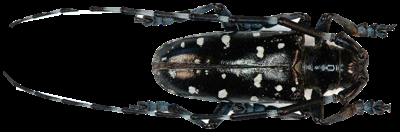
\includegraphics[width=0.92\linewidth]{figures/habitus_alb.png}\par\leg{\emph{A. glabripennis} (ALB)}\end{minipage}\hfill
\begin{minipage}[t]{0.49\linewidth}\centering
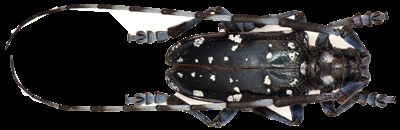
\includegraphics[width=0.92\linewidth]{figures/habitus_clb.png}\par\leg{\emph{A. chinensis} (CLB) · illustrations : fascicule de TP}\end{minipage}}

\vspace{16mm}
\bloc{Méthode}{%
\begin{tikzpicture}[font=\fontsize{23}{27}\selectfont,
  etape/.style={draw=theme,line width=1.5pt,fill=white,rounded corners=4mm,align=center,minimum height=36mm,text width=66mm,inner sep=6pt},
  fl/.style={-{Latex[length=6mm]},theme,line width=2.5pt}]
  \node[etape] (a) at (0,0) {Piégeage,\\extraction d'ADN};
  \node[etape] (b) at (95mm,0) {PCR et\\séquençage du COI};
  \node[etape] (c) at (190mm,0) {Alignement avec\\des séquences\\de référence};
  \node[etape,fill=theme!10] (d) at (285mm,0) {Réseaux\\d'haplotypes\\(R, \emph{pegas})};
  \foreach \u/\v in {a/b,b/c,c/d} \draw[fl] (\u) -- (\v);
\end{tikzpicture}

Le COI est un gène mitochondrial, transmis par la mère : deux individus qui portent le même haplotype (séquence identique) peuvent venir de la même population. Jeux de données : 148 séquences d'ALB (360 pb) et 47 de CLB (395 pb), de France, d'Europe, d'Asie et d'Amérique du Nord.}
\end{minipage}\hfill
\begin{minipage}[t]{285mm}
\bloc{Foyers en France}{\centering
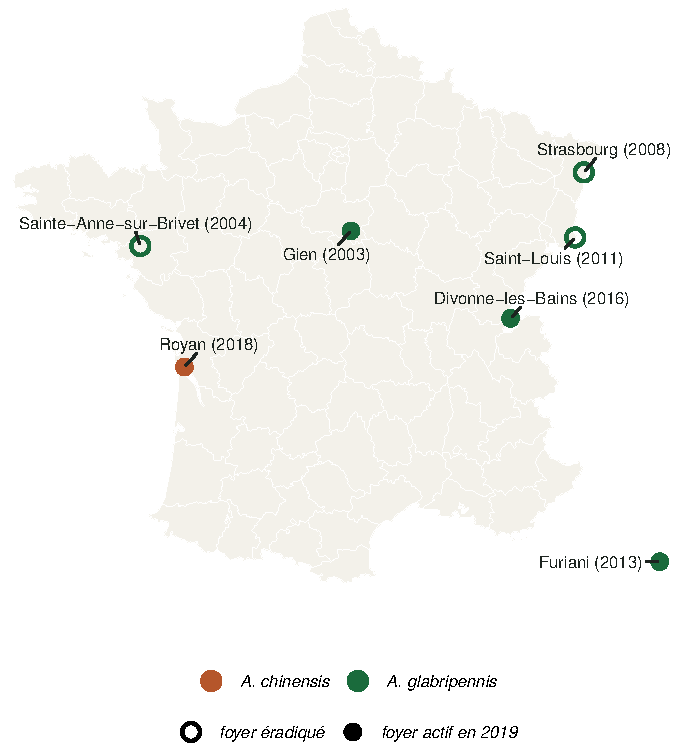
\includegraphics[width=\linewidth]{figures/carte_foyers.pdf}\par
\leg{Foyers détectés de 2003 à 2018 et leur statut en 2019.}}
\end{minipage}

\vspace{24mm}
% ---------- Rangee 3 : resultats
\bloc{Résultats}{%
\begin{minipage}[t]{368mm}
\cle{\bfseries\color{theme}ALB : deux lignées en France}\par
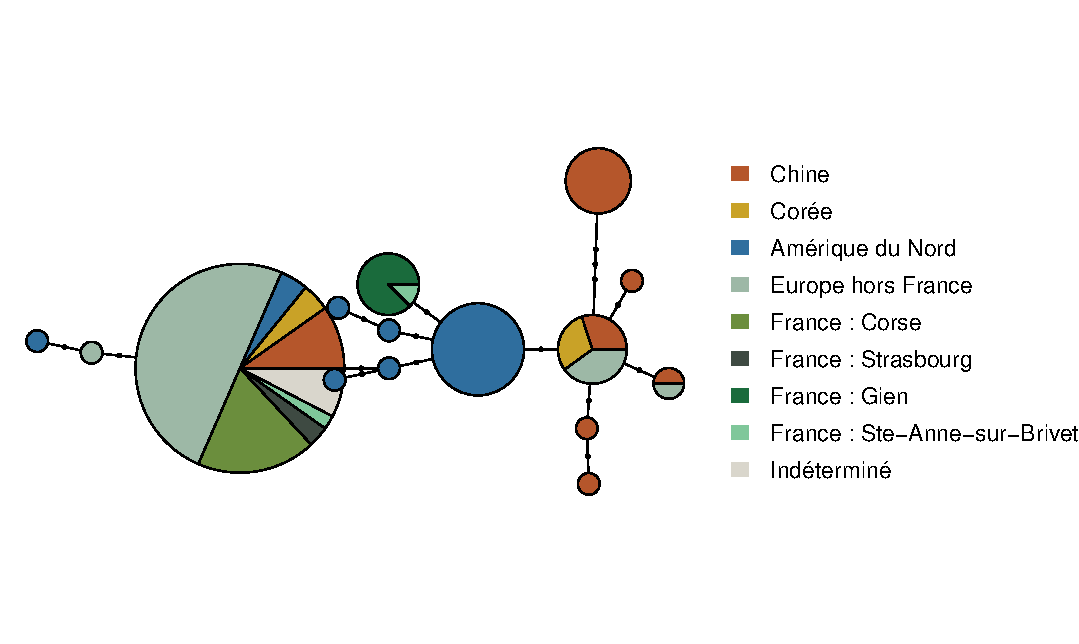
\includegraphics[width=\linewidth]{figures/reseau_alb.pdf}\par
\begin{itemize}
\item Les 7 individus de \textbf{Gien} portent un haplotype \textbf{propre à ce foyer}, partagé seulement avec Sainte-Anne-sur-Brivet. Il est à 1 mutation de l'haplotype dominant en Amérique du Nord, et à 2 des haplotypes chinois et coréens.
\item \textbf{Corse, Strasbourg} et la plupart des foyers européens partagent l'haplotype le plus fréquent, présent aussi en Chine.
\end{itemize}
\end{minipage}\hfill
\begin{minipage}[t]{368mm}
\cle{\bfseries\color{rouille}CLB : Royan relié à la Chine, pas à l'Italie}\par
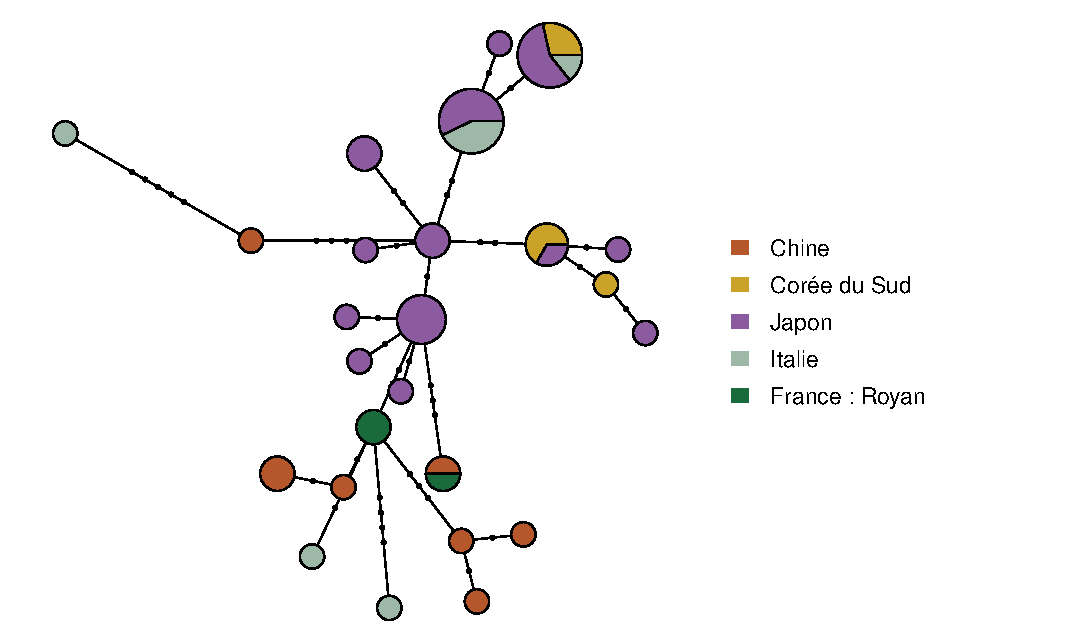
\includegraphics[width=\linewidth]{figures/reseau_clb.pdf}\par
\begin{itemize}
\item Les individus de \textbf{Royan} partagent leur haplotype avec la Chine (Shandong) ou en sont à 1 mutation (Anhui).
\item Les foyers \textbf{italiens} portent des haplotypes japonais ou sont isolés : ils ne sont pas la source de Royan.
\end{itemize}
\end{minipage}
\leg{Réseaux d'haplotypes : chaque cercle est un haplotype, de surface proportionnelle au nombre d'individus et coloré selon leur origine ; chaque trait sur une branche est une mutation.}}

\vspace{18mm}
% ---------- Rangee 4 : conclusion + references
\begin{minipage}[t]{470mm}
\bloc{Conclusion}{%
\begin{itemize}
\item Les capricornes asiatiques sont arrivés en France \textbf{par plusieurs introductions indépendantes}, et non par une seule vague.
\item Royan est une introduction \textbf{directe depuis la Chine}. Le foyer de Gien pourrait venir d'Amérique du Nord, conformément à l'effet « tête de pont » montré pour l'ALB \parencite{javal2019}, mais une mutation ne suffit pas à le prouver.
\item Le COI est court et maternel : il faut des marqueurs plus résolutifs (microsatellites, génomique) pour trancher. La détection précoce reste la clé : trois foyers ont été éradiqués, et des chiens détecteurs appuient désormais la surveillance, comme à Royan \parencite{anses2019}.
\end{itemize}}
\end{minipage}\hfill
\begin{minipage}[t]{258mm}
\bloc{Références}{\fontsize{22}{28}\selectfont
\printbibliography[heading=none]
\vspace{4pt}{\color{gris}Données : fascicule de TP « Histoire évolutive et structuration génétique des populations » (G. Roux, 2020). Analyses refaites en 2026 sous R.}}
\end{minipage}

\end{minipage}
\end{document}
